\documentclass[11pt]{article}

\newcommand{\numpy}{{\tt numpy}}    % tt font for numpy

\topmargin -.9in
\textheight 9in
\oddsidemargin -.25in
\evensidemargin -.25in
\textwidth 7in

\setlength\parindent{0pt}

\usepackage{amsmath,amsthm,amsfonts,amssymb,amscd}
\usepackage{lastpage}
\usepackage{enumerate}
\usepackage{fancyhdr}
\usepackage{mathrsfs}
\usepackage{xcolor}
\usepackage{graphicx}
\usepackage{listings}
\usepackage{hyperref}
\usepackage{enumitem}
\usepackage{float}
\usepackage{fancyvrb}
\usepackage{tabularx}
\usepackage{multicol}
\usepackage{picture}
\begin{document}
\graphicspath{{./figures/}}
% ========== Edit your name here
\author{Palle Morris e1160346\\ Elmenreich Jan e01526208\\ Holzberger Fabian e11921655 }
\title{Machine Learing Exercise 0}
\maketitle

%\medskip


\section{Introduction}
Two datasets are analyzed, one for classification and a second one for regression. The datasets were chosen such that they have different characteristics. The characteristics and more information about the datasets is listed in the table [\ref{tab:char1}].
\begin{table}[H]
\begin{tabularx}{1.0\linewidth}{XXX}
\hline
Characteristic 		& Mammographic Mass 	& House sales   \\
Data Type 		& Multivariate 	& Multivariate \\
Attribute Type  	& Integer  & Integer, String, Real\\
Associated Tasks	& Classification & Regression \\
Number of instances     & 961 		 & 21436\\
Number of Attributes    & 6 		& 20\\
Missing Values 		& Yes 		& No \\
\hline
\end{tabularx}
\label{tab:char1}
\caption{Characteristics of the datasets of choice}
\end{table}

We call the mammographic mass dataset and the house sales dataset, dataset 2. Dataset1 is used for classification and dataset 2 is used for regression. They both are multivariate wherein the difference can be seen in their dimensionality which is the number of attributes. Here dataset 2 has about 3 times higher dimesnionality than dataset 1. Moreover, dataset 2 has a wider variety of attribute types with integer, strings and real numbers where dataset 1 contains merely integers. Additionally, dataset 2 has about 20 times more instances than dataset 1 and dosent contain any missing values which dataset 1 does.

%\newpage

\section{Mammographic Dataset}
This dataset includes 6 Attributes, we summarize and explain them below

\begin{multicols}{2}
\begin{itemize}
\item \texttt{BI-RADS} Integer (non-predictive)\\
 BI-RADS assessment ranging from 1 (definitely benign)
to 5 (highly suggestive of malignancy). Can be an indication of how well a CAD system performs compared to the radiologists.
\columnbreak
\item \texttt{Serverity} Bool (target) \\
classification by 1 for benign or 0 for malignant
\item \texttt{Age} Integer  \\
Age of the specimen
\end{itemize}
\begin{itemize}
\item \texttt{Shape} Integer  \\
mass shape: round=1 oval=2 lobular=3 irregular=4 (nominal) 
\item \texttt{Margin} Integer  \\
mass margin: circumscribed=1 microlobulated=2 obscured=3 ill-defined=4 spiculated=5 
\item \texttt{Density} Integer  \\
mass density: high=1 iso=2 low=3 fat-containing=4
\end{itemize}
\end{multicols}

The missing values per attribute can be found table[\ref{tab:mamm1}]:

\begin{table}[H]
\begin{tabularx}{1.0\linewidth}{XXXXXX}
\hline
BI-RADS & Age &Shape &Margin & Density & Serverity  \\
\hline
2 & 5 & 31 & 48 & 76 & 0
\end{tabularx}
\label{tab:mamm1}
\caption{Missing values for mammograph dataset}
\end{table}

While inspecting the dataset, one instance with a BI-RADS value of 55 was found which, is an error since the range of this attribute is 5 at maximum. We correct is to the value of 5. 

The distributions of the dataset attributes can be found in figure [\ref{fig:Mamm}].

\begin{figure}[H]\center
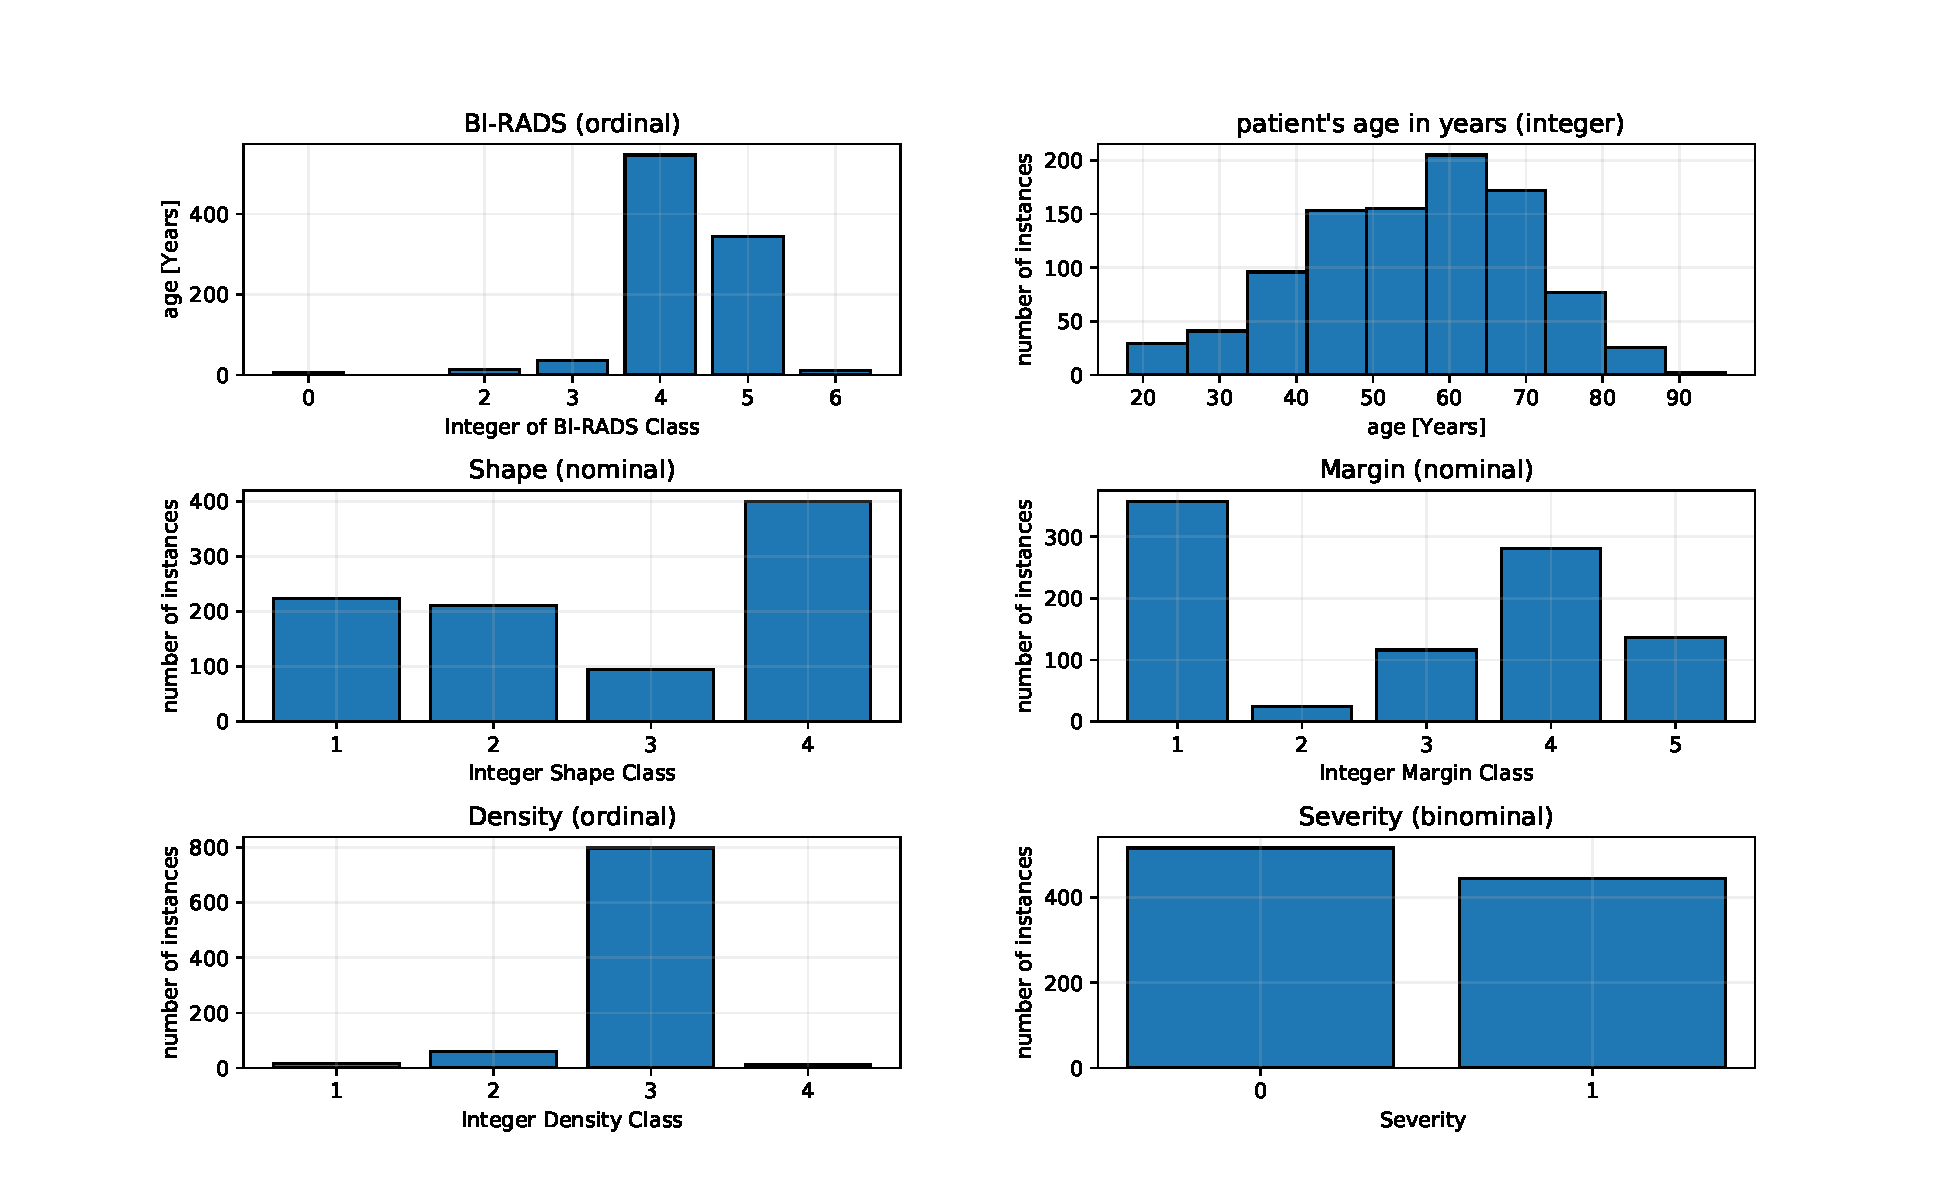
\includegraphics[width=0.8\linewidth]{Mammograph.pdf}
\caption{Histogramms of mammograpic dataset attributes}
\label{fig:Mamm}
\end{figure}

In the figure we see that the target attribute severity is binomial. The severe cases are 445 where the non-severe cases are 516 which is slightly not equal. In the BI-RADS attribute that contains ordinal values most values are in class 4 with about 500 followed by class 5 with about 350 values. It can be seen that the age (integer) of the patients is approximately normal distributed around the age 60 with a range of 20 to 90 years. The age is represented as integer value. For the shape attribute (ordinal) class 4 occurs is dominant with about 400 instances followed by class 1 and 2 with slightly more than 200 instances each and class 3 with 100 instances. Next in the margin (ordinal) attribute we see a range of 5 represented classes. Here class 1 and 4 are dominant with about 400 instances for the former and about 300 for the latter one. Lastly in the density (ordinal) attribute only class 3 shows dominance with about 800 occurrences where the other classes 1,2 and 3 occur in less than 100 instances.

\newpage
\section{House sales Dataset}
This dataset contains $20$ attributes + \texttt{id}, which we will not count as an attribute. Our target attribute will be, as so often the \texttt{price}
\begin{multicols}{2}
\begin{itemize}
\item \texttt{Price} Real (target) \\
Price of each home sold
\item \texttt{Date} String\\
Date of the home sale 
\item \texttt{Bedrooms} Integer\\
Number of bedrooms
\item \texttt{Bathrooms} Real\\
Number of Bathrooms
\item \texttt{Sqft\_living} Integer\\
Square footage of the apartments interior living space
\item \texttt{Sqft\_lot} Integer\\
Square footage of the land space
\item \texttt{Floors} Real\\
Number of floors
\item \texttt{Waterfront} Integer\\
A dummy variable for whether the apartment was overlooking the waterfront or not
\item \texttt{View} Integer\\
An index from $0$ to $4$ of how good the view of the property was
\item \texttt{Condition} Integer\\
An index from $1$ to $5$ on the condition of the apartment
\columnbreak
\item \texttt{Grade} Integer\\
An index from $1$ to $13$, where $1-3$ falls short of the building construction and design, $7$ has an average level of construction and design, and $11-13$ have a high quality level of construction and design
\item \texttt{Sqft\_Above} Integer\\
The square footage of the interior housing space that is above ground level
\item \texttt{Sqft\_basement} Integer\\
The square footage of the interior housing space that is below ground level
\item \texttt{Yr\_built} Integer\\
The year the house was initially built
\item \texttt{Yr\_renovated} Integer\\
The year of the house's last renovation
\item \texttt{Zipcode} Integer\\
What zipcode area the house is in
\item \texttt{Lat} Real\\
Latitude 
\item \texttt{Long} Real\\
Longitude
\item \texttt{Sqft\_living15} Integer\\
The square footage of interior housing living space for the nearest $15$ neighbors
\item \texttt{Sqft\_lot15} Integer\\
The square footage of the land lots of the nearest $15$ neighbors
\end{itemize}
\end{multicols}
In figure [\ref{fig:HistrogrammsHouses}] we can see the distribution of the target and other attributes.
\begin{figure}[H]
\begin{picture}(400,390)
\put(0,180){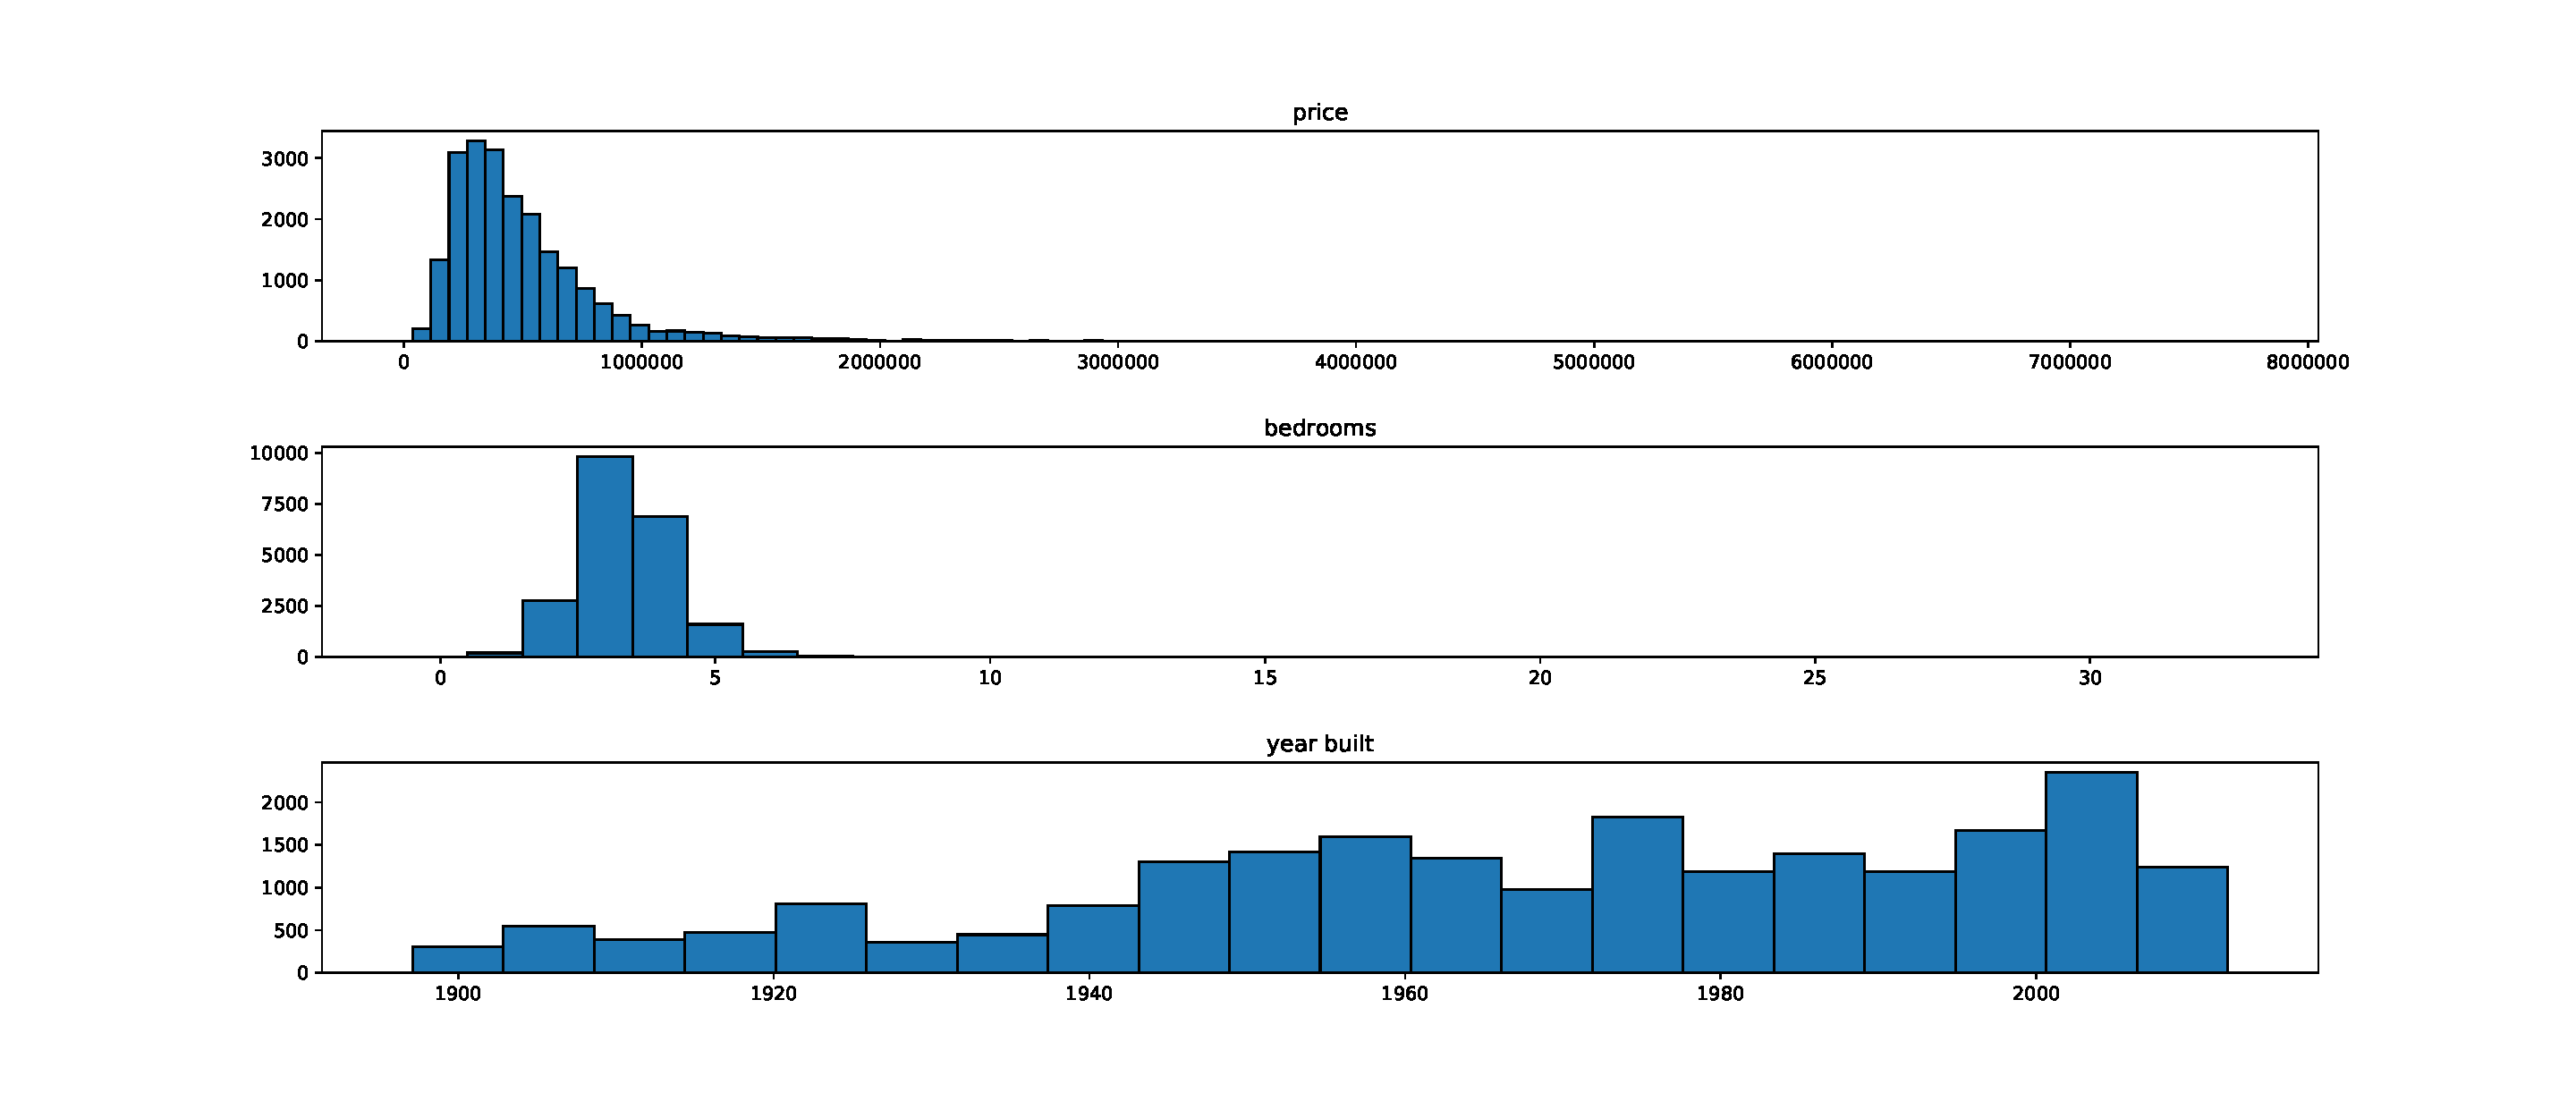
\includegraphics[width=1.0\linewidth]{HistogrammHouses1.pdf}}
\put(0,-20){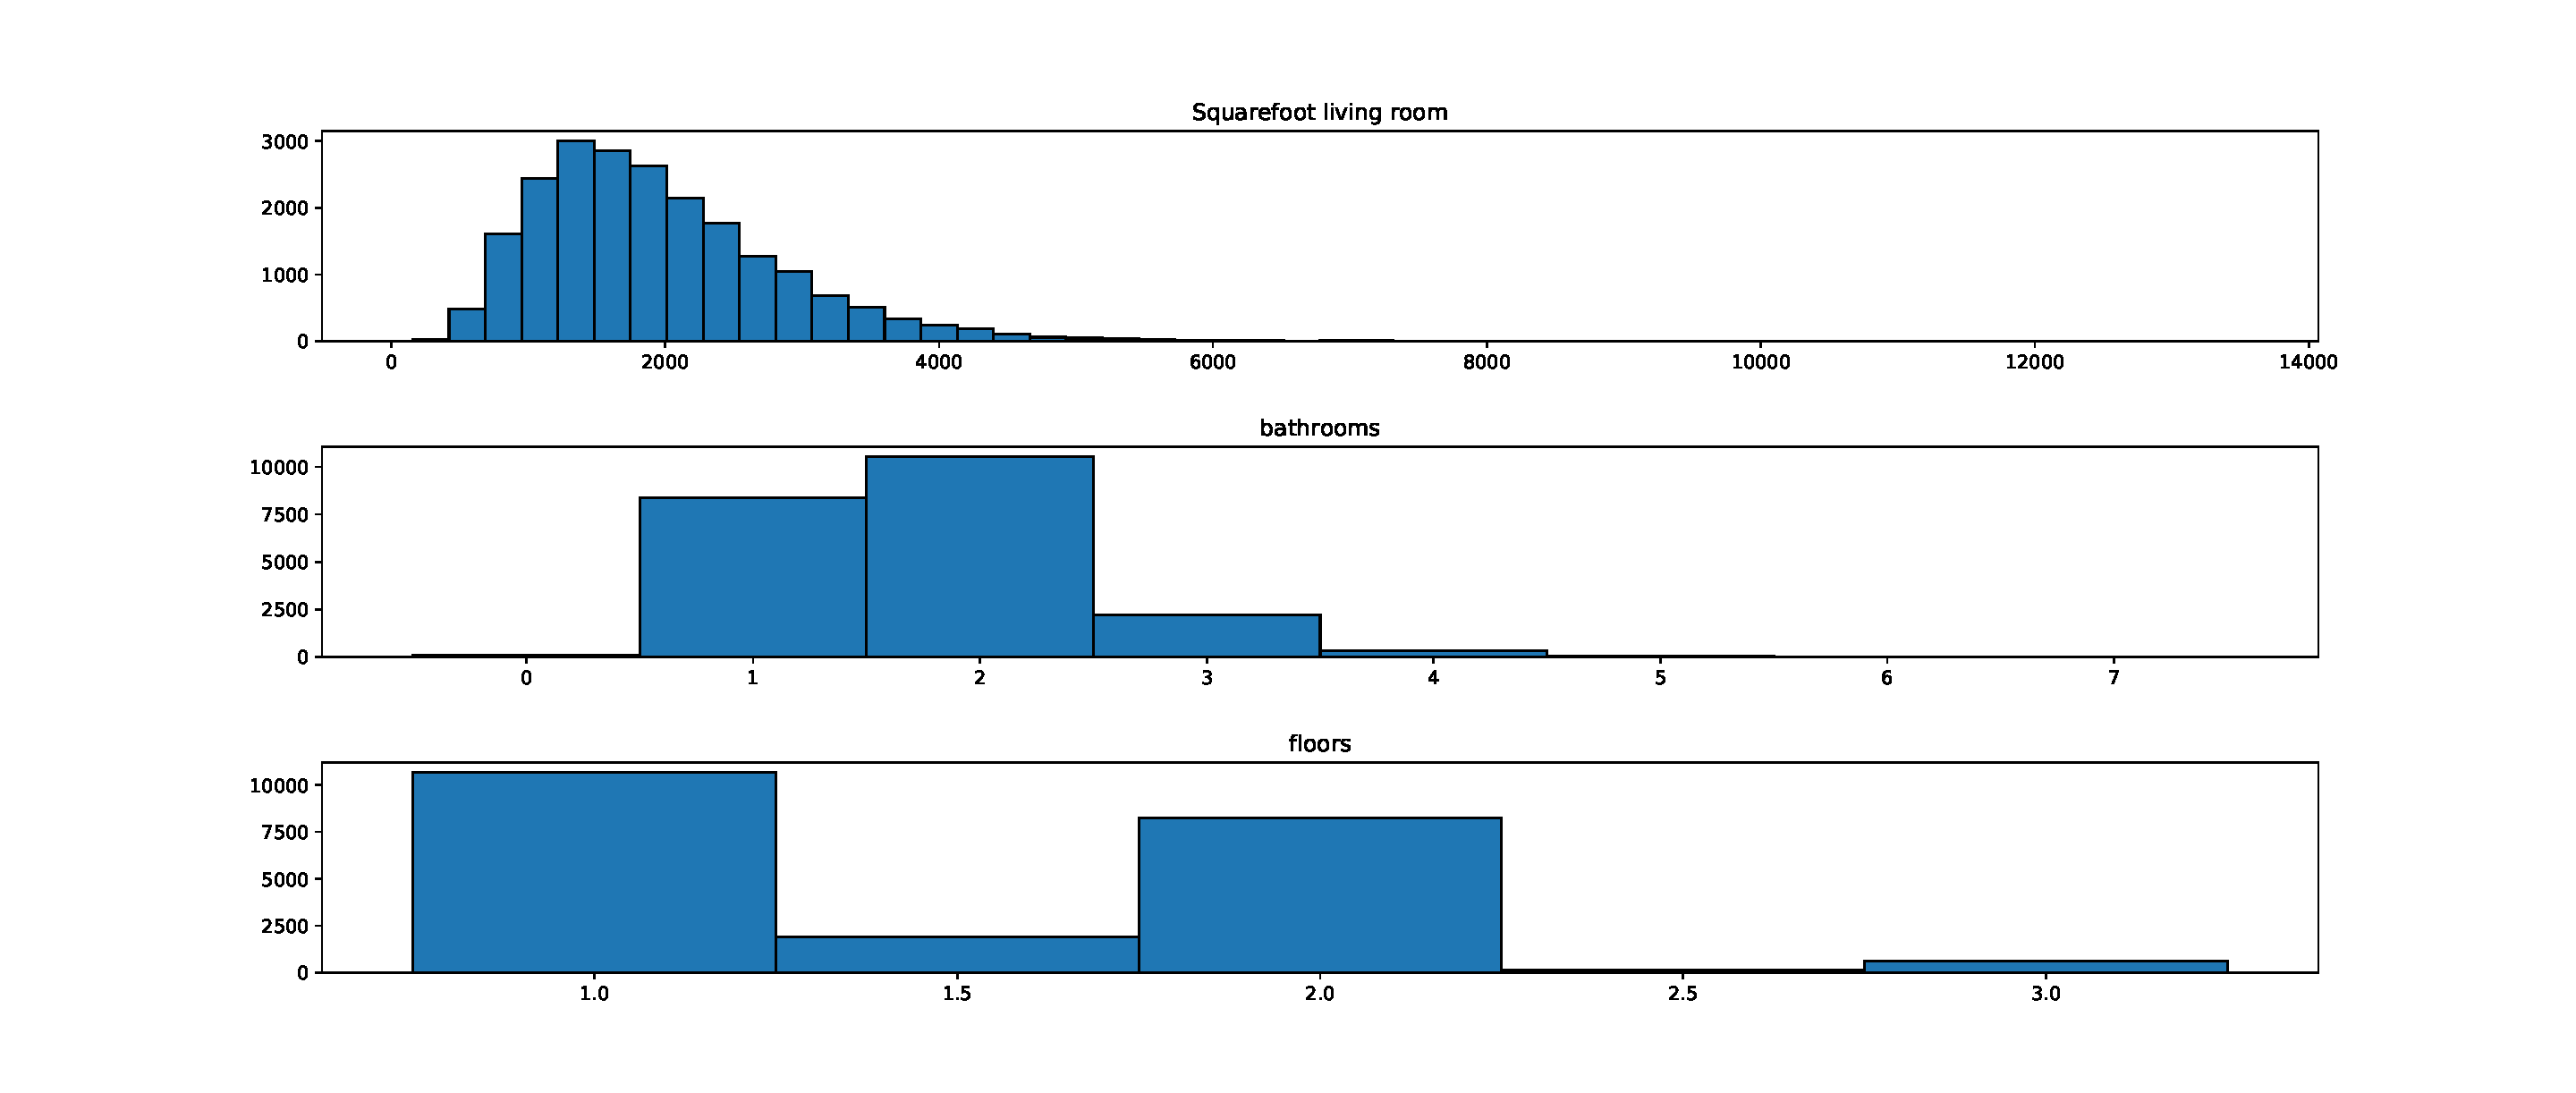
\includegraphics[width=1.0\linewidth]{HistogrammHouses2.pdf}}
\end{picture}
\caption{Histogramms of attributes}
\label{fig:HistrogrammsHouses}
\end{figure}
\end{document}
\grid
\grid
